\documentclass[journal,10pt]{IEEEtran}

\usepackage{fontspec}
\usepackage[spanish,es-nodecimaldot]{babel}
\usepackage{graphicx}
\usepackage{hyperref}
\usepackage{cite}
\usepackage{amsmath,amssymb,amsfonts}
\usepackage{algorithmic}
\usepackage{textcomp}
\usepackage{xcolor}
\usepackage{booktabs}
\usepackage{listings}

\graphicspath{{images/}}

\lstset{
  basicstyle=\ttfamily\small,
  breaklines=true,
  frame=single,
  backgroundcolor=\color{gray!10}
}

\begin{document}

\title{Servicio Administrado de Páginas y Aplicaciones Web (HTTPaaS) en Entorno Local Virtualizado}

\author{Estudiantes del Curso de Computación en la Nube\\
\IEEEmembership{Facultad de Ingeniería}\\
Universidad Tecnológica de Pereira\\
Noviembre de 2026}

\maketitle

\begin{abstract}
Este documento describe el diseño, la implementación y la validación de un servicio administrado de servidores HTTP (HTTPaaS) desplegado sobre un entorno local virtualizado con Oracle VirtualBox, Apache Web Server y Bind9. La solución orquestada en Golang permite a los usuarios aprovisionar de forma desatendida instancias web a partir de discos en modo multiconexión, actualizando dinámicamente los registros de un servidor DNS local y desplegando paquetes web comprimidos, simulando las capacidades de plataformas de nube como servicio (IaaS/PaaS).
\end{abstract}

\begin{IEEEkeywords}
Computación en la nube, HTTPaaS, VirtualBox, discos multiconexión, Bind9, DNS dinámico, Golang, arquitectura hexagonal.
\end{IEEEkeywords}

\section{Introducción}

El crecimiento sostenido de los modelos de computación en la nube ha transformado la manera en que las organizaciones despliegan, administran y escalan aplicaciones de software. Los modelos de Infraestructura como Servicio (IaaS) y Plataforma como Servicio (PaaS) permiten a los usuarios aprovisionar capacidad de cómputo y pilas de ejecución bajo demanda sin gestionar la complejidad del hardware físico subyacente.

En este contexto, el presente proyecto desarrolla un sistema de Servicio Administrado de Servidores HTTP (HTTPaaS) implementado en un entorno local virtualizado. La plataforma combina tecnologías de virtualización con Oracle VirtualBox, resolución de nombres dinámica con Bind9 y un motor orquestador desarrollado en Golang bajo el patrón de arquitectura hexagonal. 

A través de una interfaz gráfica web centralizada, los usuarios pueden solicitar instancias de servidores web Apache proporcionando un nombre de host deseado y un archivo comprimido (\texttt{.zip}) con el contenido web a publicar. El sistema automatiza completamente el ciclo de vida: creación de máquinas virtuales a partir de discos en modo multiconexión, asignación de red, actualización de zonas DNS y despliegue del contenido.


\section{Marco Teórico}

\subsection{Virtualización y Discos en Modo Multiconexión}
La virtualización completa permite ejecutar múltiples sistemas operativos invitados de forma aislada sobre un único hipervisor de tipo 2, como Oracle VirtualBox \cite{virtualbox2024}. Para optimizar el aprovisionamiento de máquinas homogéneas y reducir el consumo de almacenamiento, VirtualBox ofrece la modalidad de almacenamiento \textit{multiattach} (multiconexión).

En el modo multiconexión, una imagen base (\texttt{ApacheServer.vdi}) se comparte entre múltiples máquinas virtuales en modo de solo lectura. Cuando una máquina virtual escribe en el disco, los cambios se desvían de manera transparente a una imagen diferencial (\textit{differencing image}) exclusiva para esa instancia. Esta técnica agiliza la clonación casi instantánea de servidores sin duplicar el sistema operativo base.

\subsection{Servicio de Nombres de Dominio y DNS Dinámico (Bind9)}
El Sistema de Nombres de Dominio (DNS) es un componente crítico en la infraestructura de redes \cite{albitz2001dns}. Para evitar la edición manual y el reinicio continuo del demonio \texttt{named}, se utiliza la especificación de actualización dinámica (RFC~2136) \cite{rfc2136}, que permite a la capa de orquestación insertar y revocar registros de tipo A en tiempo de ejecución, manteniendo coherencia con la zona local administrada por Bind9.

\subsection{Arquitectura Hexagonal (Puertos y Adaptadores)}
Propuesta por Alistair Cockburn \cite{cockburn2005hexagonal}, la arquitectura hexagonal persigue el desacoplamiento de la lógica de dominio respecto a las dependencias de infraestructura y protocolos de entrada/salida. El núcleo permanece puro y agnóstico a las herramientas externas mediante contratos formales de puertos (interfaces), facilitando la testabilidad unitaria con dobles de prueba y el mantenimiento a largo plazo.

\subsection{Contrato REST y Desarrollo Guiado por Pruebas}
La exposición de capacidades de aprovisionamiento mediante una API REST con contrato OpenAPI permite separar el orquestador de sus clientes (interfaz web u otros consumidores) y documentar de forma verificable los recursos, parámetros y respuestas. Complementariamente, el desarrollo guiado por pruebas (TDD) y las pruebas de contrato sobre interfaces y módulos reducen regresiones al validar invariantes de dominio, orquestación y contratos de presentación antes y durante la implementación.


\section{Diseño de la Solución}

\subsection{Arquitectura del Sistema}
La solución se compone de tres capas arquitectónicas:
\begin{enumerate}
    \item \textbf{Capa Primaria (Controladores y Presentación):} Servidor HTTP en Go que expone una interfaz gráfica HTML/CSS/JS y una API REST compatible con OpenAPI 3.0.
    \item \textbf{Capa de Aplicación y Dominio:} Servicios orquestadores transaccionales que coordinan la creación de recursos y gestionan fallos mediante rutinas de compensación (\textit{rollback}).
    \item \textbf{Capa Secundaria (Adaptadores de Infraestructura):} Implementaciones concretas de los puertos que invocan la interfaz de línea de comandos de VirtualBox (\texttt{VBoxManage}), utilitarios DNS (\texttt{nsupdate} o SSH sobre Bind9) y utilidades de transferencia de archivos.
\end{enumerate}

\subsection{Topología de Red}
Se define una red interna virtual (\texttt{cloudnet}) bajo el segmento IPv4 \texttt{192.168.10.0/24}:
\begin{itemize}
    \item \textbf{Host anfitrión:} \texttt{192.168.10.1} (interfaz Host-Only).
    \item \textbf{Servidor DNS (\texttt{ns}):} \texttt{192.168.10.10/24}, administrando la zona \texttt{cloud.local.}.
    \item \textbf{Instancias dinámicas:} Direcciones en el rango \texttt{192.168.10.30} a \texttt{192.168.10.254}.
\end{itemize}

\begin{figure}[htbp]
\centering
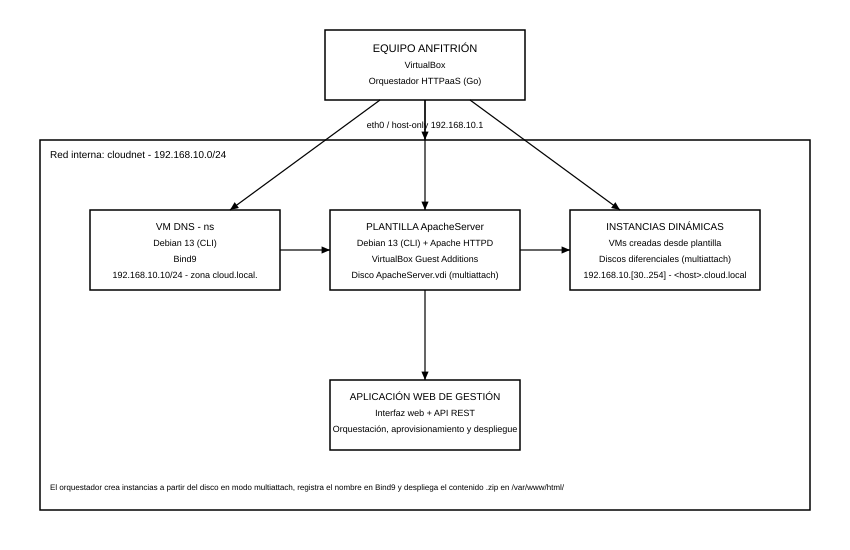
\includegraphics[width=\linewidth]{escenario.svg}
\caption{Diagrama de escenario: topología de red y componentes del entorno HTTPaaS.}
\label{fig:escenario}
\end{figure}



\subsection{Vista de Procesos: Flujo de Aprovisionamiento}
El aprovisionamiento se realiza de forma automatizada y transaccional, garantizando la coherencia entre los componentes de virtualización, DNS y despliegue web.

\begin{figure}[htbp]
\centering
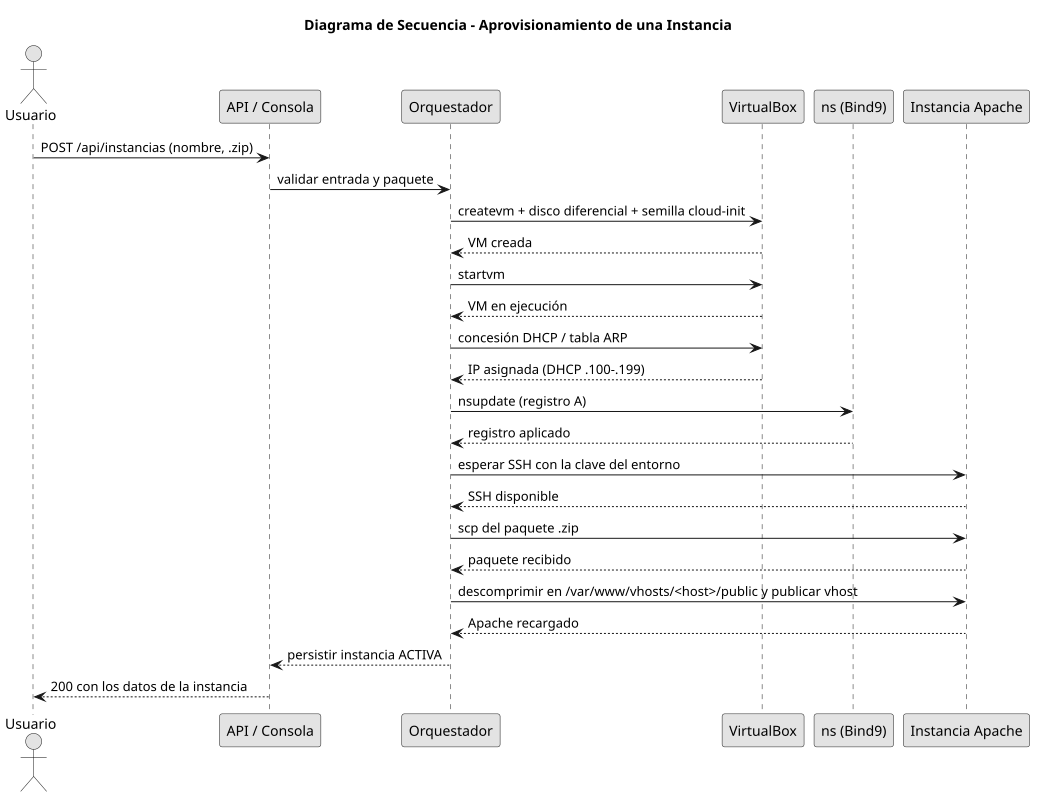
\includegraphics[width=\linewidth]{secuencia.svg}
\caption{Diagrama de secuencia del flujo de aprovisionamiento de instancias HTTPaaS.}
\label{fig:secuencia}
\end{figure}

\subsection{Manejo de Compensaciones (Rollback)}
Si alguna etapa del aprovisionamiento falla, el orquestador ejecuta rutinas de compensación inversa para mantener la infraestructura en un estado consistente:
\begin{itemize}
    \item Si falla el registro DNS: se destruye la máquina virtual creada en VirtualBox.
    \item Si falla el despliegue del archivo \texttt{.zip}: se elimina el registro DNS correspondiente y se destruye la máquina virtual creada en VirtualBox.
\end{itemize}

\section{Implementación}

\subsection{Estructura del Backend en Go}
El backend se implementó en Go siguiendo arquitectura hexagonal y un flujo de trabajo \emph{docs $\rightarrow$ test $\rightarrow$ implementación}. La organización principal del código es:
\begin{itemize}
    \item \texttt{cmd/server}: punto de entrada, configuración por \textit{flags}, ensamblado de dependencias (inyección en \texttt{main}) y exposición HTTP.
    \item \texttt{internal/core/domain}: modelos, normalización de nombres y reglas/invariantes del dominio (por ejemplo, validación de \textit{hostname}/FQDN).
    \item \texttt{internal/core/ports}: contratos de infraestructura (\texttt{Executor}, \texttt{Hypervisor}, \texttt{DnsProvider}, \texttt{Deployer}, \texttt{Repository}) y el puerto transversal de observabilidad (\texttt{EventLogger}).
    \item \texttt{internal/adapters}: implementaciones concretas (\texttt{localproc} para ejecución de procesos, \texttt{vbox} para \texttt{VBoxManage}, \texttt{bind9} para registro/consulta DNS, \texttt{deployer} para despliegue y \texttt{filestore} para persistencia).
    \item \texttt{internal/services}: orquestación transaccional del aprovisionamiento/eliminación y políticas de compensación.
    \item \texttt{internal/handlers}: adaptadores primarios HTTP (instancias, DNS, salud, logs, middleware de \textit{logging}/CORS/recuperación y respuestas JSON).
    \item \texttt{internal/logging}: modelo de eventos y \textit{broker} en memoria (anillo acotado y suscripción a canales) que implementa \texttt{ports.EventLogger} y sirve de puente con el paquete \texttt{log} estándar.
    \item \texttt{web}: interfaz de usuario estática servida por el orquestador.
\end{itemize}

\subsection{Orquestación, Infraestructura y Concurrencia}
El aprovisionamiento coordina la creación/arranque de la VM, la obtención de IP, el registro DNS, el despliegue del \texttt{.zip} y la persistencia del estado. Ante fallos, el orquestador aplica compensaciones para evitar inconsistencias (revocación DNS y destrucción/liberación de recursos según la etapa fallida).

Las operaciones sobre VirtualBox se ejecutan mediante el adaptador \texttt{vbox}, que serializa accesos críticos para mitigar condiciones de carrera asociadas al servicio \texttt{VBoxSVC} (uso de exclusión mutua). La interacción con procesos del sistema se abstrae mediante el puerto \texttt{Executor}, lo que permite aislar dependencias del host y facilitar pruebas con dobles.

\subsection{Interfaz Web Modular}
La interfaz en \texttt{web/} se implementó como un conjunto de páginas HTML (\texttt{index}, \texttt{detalle}, \texttt{dns}, \texttt{salud}, \texttt{vhosts}, \texttt{ayuda}) con componentes compartidos y reutilizables: montaje de cabecera/pie (\texttt{components.js}), panel global de eventos con estado persistido (\texttt{logs-dock.js}), utilidades comunes (\texttt{common.js}), enrutamiento por intercambio de \texttt{<main>} sin recarga completa (\texttt{router.js}) y lógica por módulo (\texttt{js/pages/*.js}).

La consola de aprovisionamiento incluye validación/ayudas de \textit{hostname}, verificación de disponibilidad, carga de contenido mediante zona de arrastre/selección para archivos \texttt{.zip}, retroalimentación de estado y confirmación de eliminación. Se incorporaron mejoras de accesibilidad y operación: navegación accesible en anchos reducidos, gestión de foco/teclado en el diálogo de eliminación, estados \texttt{aria-busy}/deshabilitado en acciones asíncronas y visualización del estado de salud consumiendo \texttt{/api/salud} (sin afirmar disponibilidad sin evidencia).

\subsection{Observabilidad: Logs Estructurados y Streaming}
La observabilidad se implementó con un \textit{broker} en memoria (\texttt{internal/logging}) que conserva un anillo acotado de eventos y notifica a los suscriptores en tiempo real. Cada evento sigue un contrato estable (\texttt{id}, \texttt{ts}, \texttt{nivel}, \texttt{componente}, \texttt{mensaje}, \texttt{campos}) y se emite desde los servicios de orquestación y desde los adaptadores de infraestructura, además de capturar la salida del paquete \texttt{log} estándar mediante un puente \texttt{io.Writer}.

Sobre ese núcleo se exponen tres operaciones: consulta filtrable del historial (\texttt{GET /api/logs} con \texttt{limit}, \texttt{nivel}, \texttt{componente} y cursor \texttt{since}), limpieza del anillo (\texttt{DELETE /api/logs}) y transmisión por Server-Sent Events (\texttt{GET /api/logs/stream}) con reanudación mediante \texttt{Last-Event-ID} o \texttt{since}, lo que evita pérdidas de eventos ante reconexiones del cliente. En el plano de seguridad, los errores internos se registran con su detalle en el \textit{broker} mientras la respuesta HTTP 500 expone un mensaje público estable, evitando filtrar trazas de infraestructura.

En la interfaz, el \textit{dock} de eventos consume el historial al abrirse y mantiene una conexión \textit{EventSource} al flujo, deduplicando por identificador; su indicador de conexión refleja los estados conectando, en vivo y reconectando.

\subsection{Calidad, Contratos y Automatización}
El proyecto define su contrato HTTP en \texttt{docs/openapi.yaml} y documenta módulos web y requisitos en \texttt{docs/}. Las pruebas unitarias cubren dominio, adaptadores, servicios y \textit{handlers}; además, se incorporaron pruebas de contrato de la interfaz web (\texttt{web/ui\_contract\_test.go}) para validar presencia de componentes, identificadores, atributos de accesibilidad y comportamientos esperados del \textit{shell} compartido. Las tareas de formato, verificación y compilación del informe se centralizan en \texttt{Taskfile.yml}.

\section{Pruebas y Evidencias}

\subsection{Pruebas Unitarias y de Integración}
Siguiendo la metodología guiada por pruebas (TDD), se implementaron pruebas unitarias sobre los casos de uso principales utilizando dobles de prueba (\textit{fakes}) para los puertos del hipervisor y del DNS. Esto garantiza que la lógica de orquestación y las rutinas de compensación ante fallos se validen de forma continua e independiente de la infraestructura física.

\subsection{Evidencias de Despliegue en Entorno Real}
A continuación se relacionan las evidencias del ciclo de vida de aprovisionamiento de las instancias solicitadas en la rúbrica del proyecto (\texttt{paisajes} y \texttt{negocios}):

\begin{figure}[htbp]
\centering
\includegraphics[width=0.9\linewidth]{captura-dashboard-vacio.png}
\caption{Panel de gestión inicial en estado vacío.}
\label{fig:dashboard_vacio}
\end{figure}

\begin{figure}[htbp]
\centering
\includegraphics[width=0.9\linewidth]{captura-formulario-subida.png}
\caption{Carga del archivo comprimido para la instancia \texttt{paisajes}.}
\label{fig:form_subida}
\end{figure}

\begin{figure}[htbp]
\centering
\includegraphics[width=0.9\linewidth]{captura-instancia-paisajes.png}
\caption{Instancia \texttt{paisajes} desplegada y visible en el panel.}
\label{fig:instancia_paisajes}
\end{figure}

\begin{figure}[htbp]
\centering
\includegraphics[width=0.9\linewidth]{captura-instancia-negocios.png}
\caption{Instancia \texttt{negocios} desplegada concurrentemente.}
\label{fig:instancia_negocios}
\end{figure}


\section{Dificultades, Mejoras y Conclusiones}

\subsection{Dificultades Técnicas}
Durante el diseño e implementación se identificaron retos relevantes:
\begin{enumerate}
    \item \textbf{Concurrencia en VirtualBox:} las invocaciones concurrentes a \texttt{VBoxManage} pueden generar condiciones de carrera con \texttt{VBoxSVC}. Se mitigó centralizando y serializando operaciones críticas en el adaptador del hipervisor.
    \item \textbf{Detección dinámica de IP:} la asignación de red en la VM no es inmediata; se requiere sondeo controlado (con espera/reintentos) apoyado en mecanismos de consulta del invitado para obtener una IP utilizable antes de registrar DNS o desplegar.
    \item \textbf{Consistencia transaccional entre subsistemas:} un fallo en DNS, IP o despliegue puede dejar recursos huérfanos. La orquestación incorpora compensaciones (\textit{rollback}) para preservar coherencia entre VM, DNS y contenido.
    \item \textbf{Contraste entre interfaz y estado real:} en consolas operativas es riesgoso mostrar estados \emph{hardcoded}. La interfaz evolucionó hacia indicadores basados en \texttt{/api/salud} y manejo explícito de estados de carga/error, aunque la verificación visual final depende de la estabilización de la UI y del laboratorio.
\end{enumerate}

\subsection{Trabajo Futuro}
\begin{itemize}
    \item Completar evidencias de laboratorio (aprovisionamiento de \texttt{paisajes}/\texttt{negocios}, resolución DNS y capturas) una vez estabilizada la interfaz.
    \item Conectar datos operativos reales a módulos evolutivos (VHosts/eventos) mediante endpoints dedicados o enriquecimiento de respuestas.
    \item Incorporar controles de cuota/recursos por instancia y endurecimiento de seguridad (validación reforzada de \texttt{.zip}, autenticación/autorización si el entorno lo requiere).
    \item Evaluar TLS/HTTPS en el entorno local y estrategias de observabilidad con correlación de eventos por operación.
\end{itemize}

\subsection{Conclusiones}
Se diseñó e implementó una base funcional de HTTPaaS que integra virtualización, DNS dinámico y orquestación en Go para automatizar el ciclo de vida de servicios HTTP en un entorno local. La arquitectura hexagonal permitió desacoplar el dominio de la infraestructura, favoreciendo pruebas automatizadas y evolución controlada. El contrato OpenAPI y la interfaz web modular proporcionan un punto de acceso coherente para el aprovisionamiento mediante archivos \texttt{.zip}, mientras que la incorporación de TDD, pruebas de contrato y consideraciones de accesibilidad/verdad operativa fortalecen la mantenibilidad. Queda pendiente la consolidación final de evidencias en el laboratorio y la estabilización visual de la interfaz para cerrar la entrega documental.


\bibliographystyle{IEEEtran}
\bibliography{ref}

\end{document}

